%%%%%%
%
% $Autor: Wings $
% $Datum: 2020-01-18 11:15:45Z $
% $Pfad: WuSt/Skript/Produktspezifikation/powerpoint/ImageProcessing.tex $
% $Version: 4620 $
%
%%%%%%


\chapter{Datenblätter}

\section{Datenübersicht}

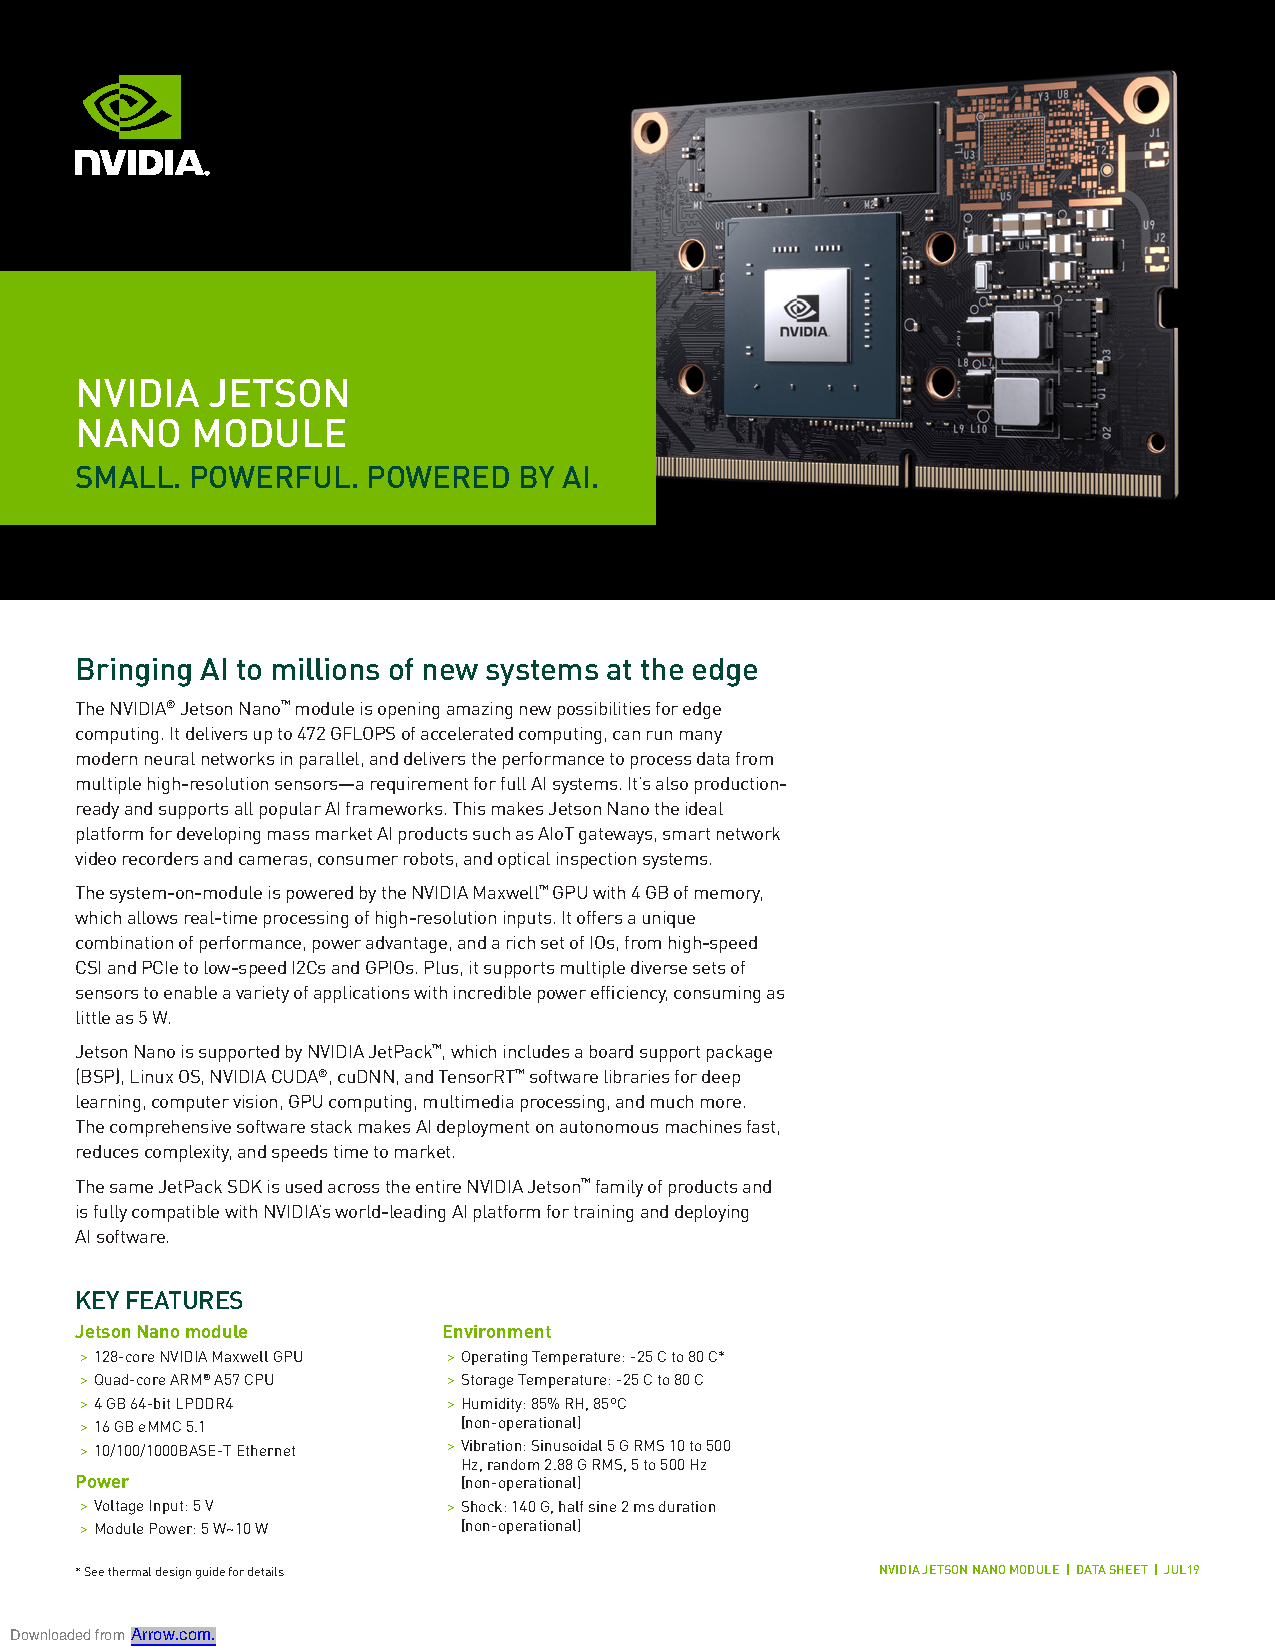
\includegraphics[width=1\textwidth,page=1]{../../MLbib/JetsonNano/jetson-nano-module-datasheet-us-1031771-r3-hr.pdf}

\includegraphics[width=1\textwidth,page=2]{../../MLbib/JetsonNano/jetson-nano-module-datasheet-us-1031771-r3-hr.pdf}


\section{Datenblatt}

\newcounter{mycounter}
\setcounter{mycounter}{1}

\whiledo {\value{mycounter} < 39}
{
\includegraphics[width=1\textwidth,page=\themycounter]{../../MLbib/JetsonNano/NVIDIAJetsonNanoDataSheet.pdf}
\stepcounter{mycounter}
\newpage
}

\section{Jetson Nano Developer Kit - User Guide}

\setcounter{mycounter}{1}

\whiledo {\value{mycounter} < 27}
{
	\includegraphics[width=1\textwidth,page=\themycounter]{../../MLbib/JetsonNano/JetsonNanoDeveloperKitUserGuide.pdf}
	\stepcounter{mycounter}
	\newpage
}


\section{Jetson Nano Developer Kit 40-Pin 	Expansion Header Configuration - Application Note}

\setcounter{mycounter}{1}

\whiledo {\value{mycounter} < 10}
{
	
\includegraphics[width=1\textwidth,page=\themycounter]{../../MLbib/JetsonNano/JetsonNanoDeveloperKit40.pdf}
	\stepcounter{mycounter}
	\newpage
}

\section{Jetson Nano Developer Kit 40-Pin Expansion Header GPIO Usage 	Considerations - 
	Application Note}

\setcounter{mycounter}{1}

\whiledo {\value{mycounter} < 13}
{
	\includegraphics[width=1\textwidth,page=\themycounter]{../../MLbib/JetsonNano/JetsonNanoDeveloperKit40II.pdf}
	\stepcounter{mycounter}
	\newpage
}
